\chapter{Theory}\label{chap:cms}


One of the most compelling questions in participle physics today is the hierarchy problem. The Randall Sundrum Kaluza Klein model proposes a solution in which the Planck scale is located on one membrane and the TeV scale a distance L away in a fourth spatial dimension. 


\section{Standard Model Particle Interactions}

Particles interact by exchanging force particles, all of which are spin-1 bosons in the Standard Model. The force particles are excitations of their corresponding fields. For the electromagnetic field, the force particle is the photon. The cross section of an interaction between particles is proportional to the scattering amplitude. In the simplest case of an electromagnetic interaction, an electron and muon collide with each other and exchange a photon. The coupling strength of the electromagnetic interaction is $e$, and the scattering amplitude is $sin^{-4}(\frac{\theta}/{2})$. This relationship to the scattering angle occurs because the mediation force particle is massless. In the weak force interactions, the mediating particle is not massless, since the mass of the $Z$ boson is 91 GeV and the mass of the $W$ boson is 80 GeV. Therefore, weak interactions are suppressed when $q^2 << {M^{2}}_{W}$.


Table \ref{fig:smtable} shows the SM particle interactions for the corresponding SM particles.

Figure \ref{fig:sm} shows the particles that are fundamental in the standard model of particles physics.
 \begin{figure}[h]
\centering
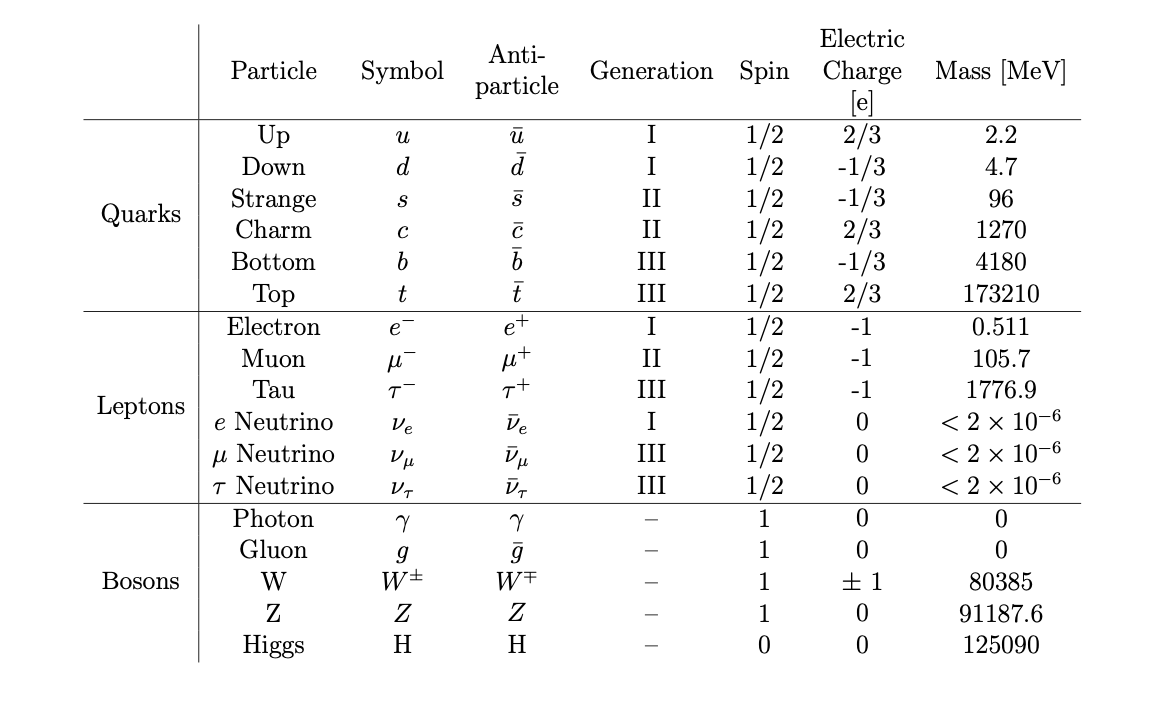
\includegraphics[width=0.8\textwidth]{figures/sm_table.png}
\caption{Table of SM particle interactions \textbf{to be replaced}.}
\label{fig:smtable}
\end{figure}


 \begin{figure}[h]
\centering
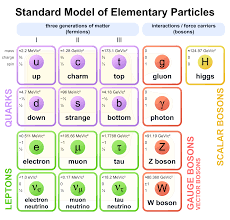
\includegraphics[width=0.8\textwidth]{figures/sm_blocks.png}
\caption{The fundamental particles in the standard model of particle physics.}
\label{fig:sm}
\end{figure}

\section{Beyond Standard Model}

One of the theories introduced to explain the hierarchy problem is the Kaluza-Klein gluon with an extra spacial dimension from the Randall-Sundrum (RS) framework. In the RS framework, there are two planes - the UV plane and the IR plane. The planck scale is located on the UV plane, and the TeV scale is located on the IR plane. The two planes interact in the fifth spacial dimension, called the “bulk”. The Kaluza-Klein gluon has a signal comparable to SM QCD background with a luminosity of 100 fb$^{-1}$, which is comparable to the 137 fb$^{-1}$ luminosity of Run 2.